\documentclass[UTF-8]{article}


\usepackage{url}
\usepackage{cite}
\usepackage[version=4]{mhchem}
\usepackage{graphicx}
\usepackage{subfigure}
\usepackage[a4paper,top=2cm,bottom=2cm,right=3cm,left=3cm,marginparwidth=1.75cm]{geometry}


\title{Template}
\author{Yan Haoming}
\date{September 27, 2024}


\begin{document}
\maketitle
\begin{abstract}
    pass now.
\end{abstract}
\textbf{Keywords: }
\section{Part One}
This is a template for convenient writing process.
The text book helps\cite{TheCell} me a lot.
We should use bibtex to compile the document,

 % Figure
 \begin{figure}
    \centering
    \subfigure[fig 1]{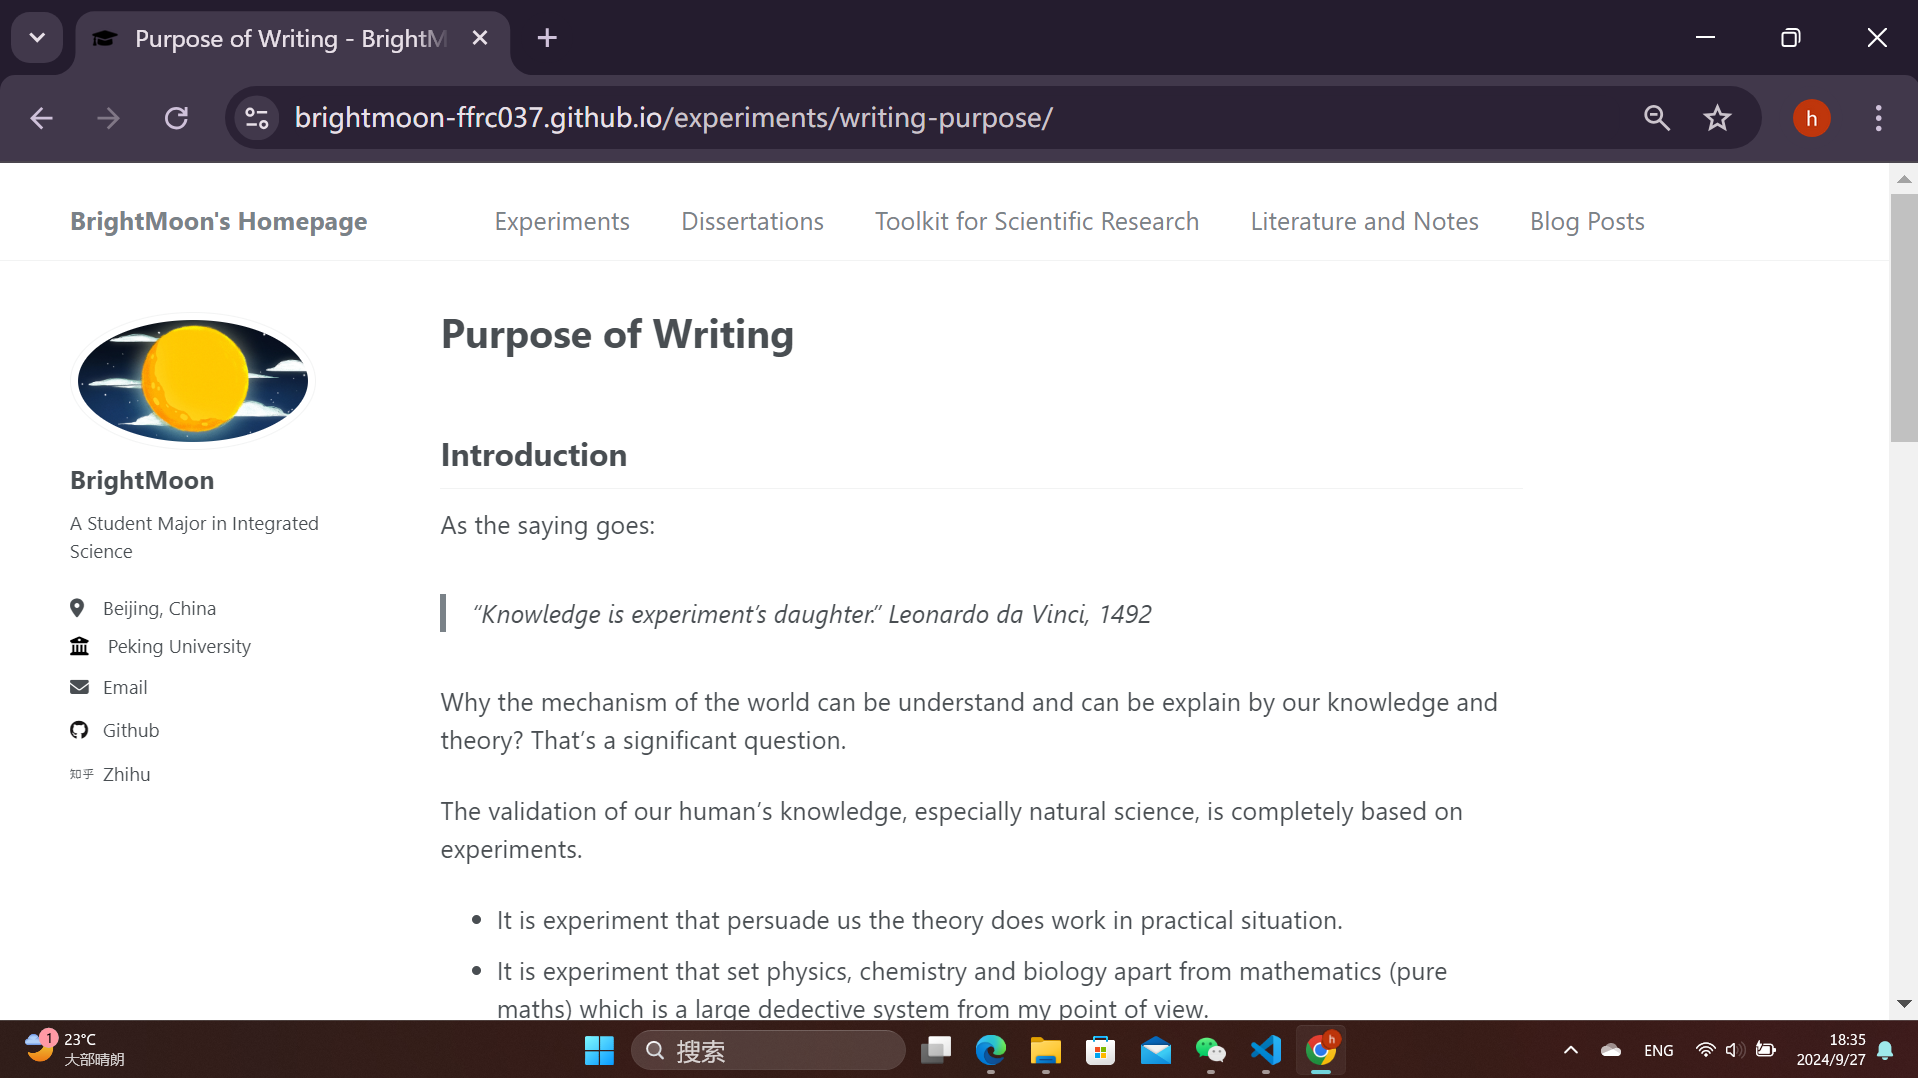
\includegraphics[width=0.7\linewidth]{../Figures/example 1.png}}
    \subfigure[fig 2]{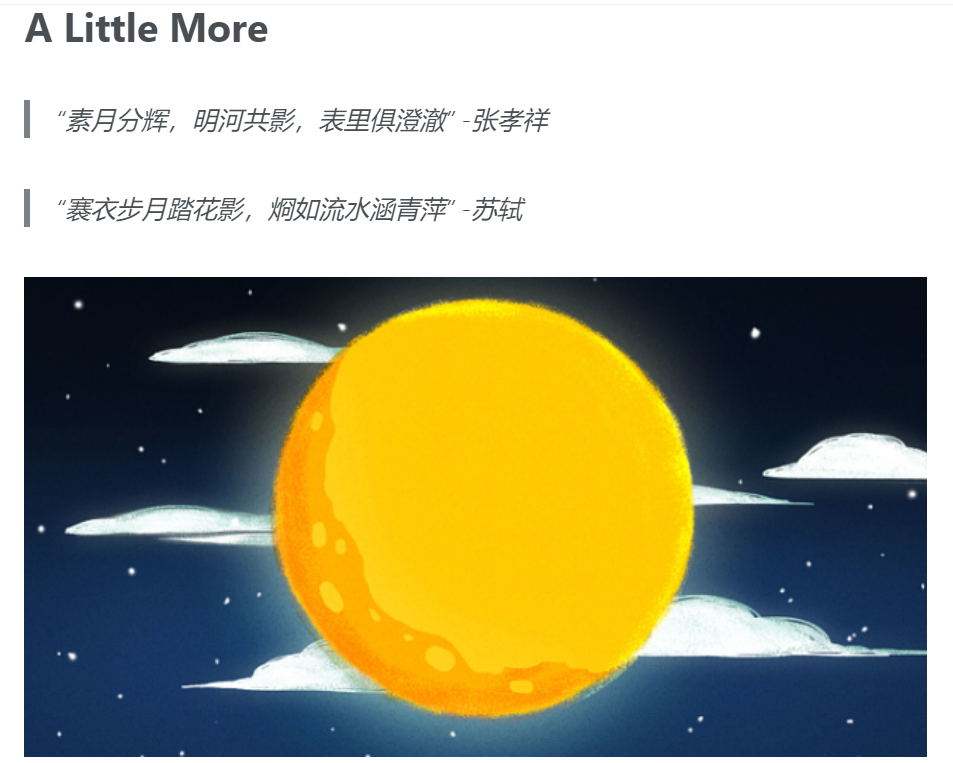
\includegraphics[width=0.7\linewidth]{../Figures/example 2.png}}
    \caption{example 1}  
    \label{example 1}
 \end{figure}

\begin{figure}
    \centering
    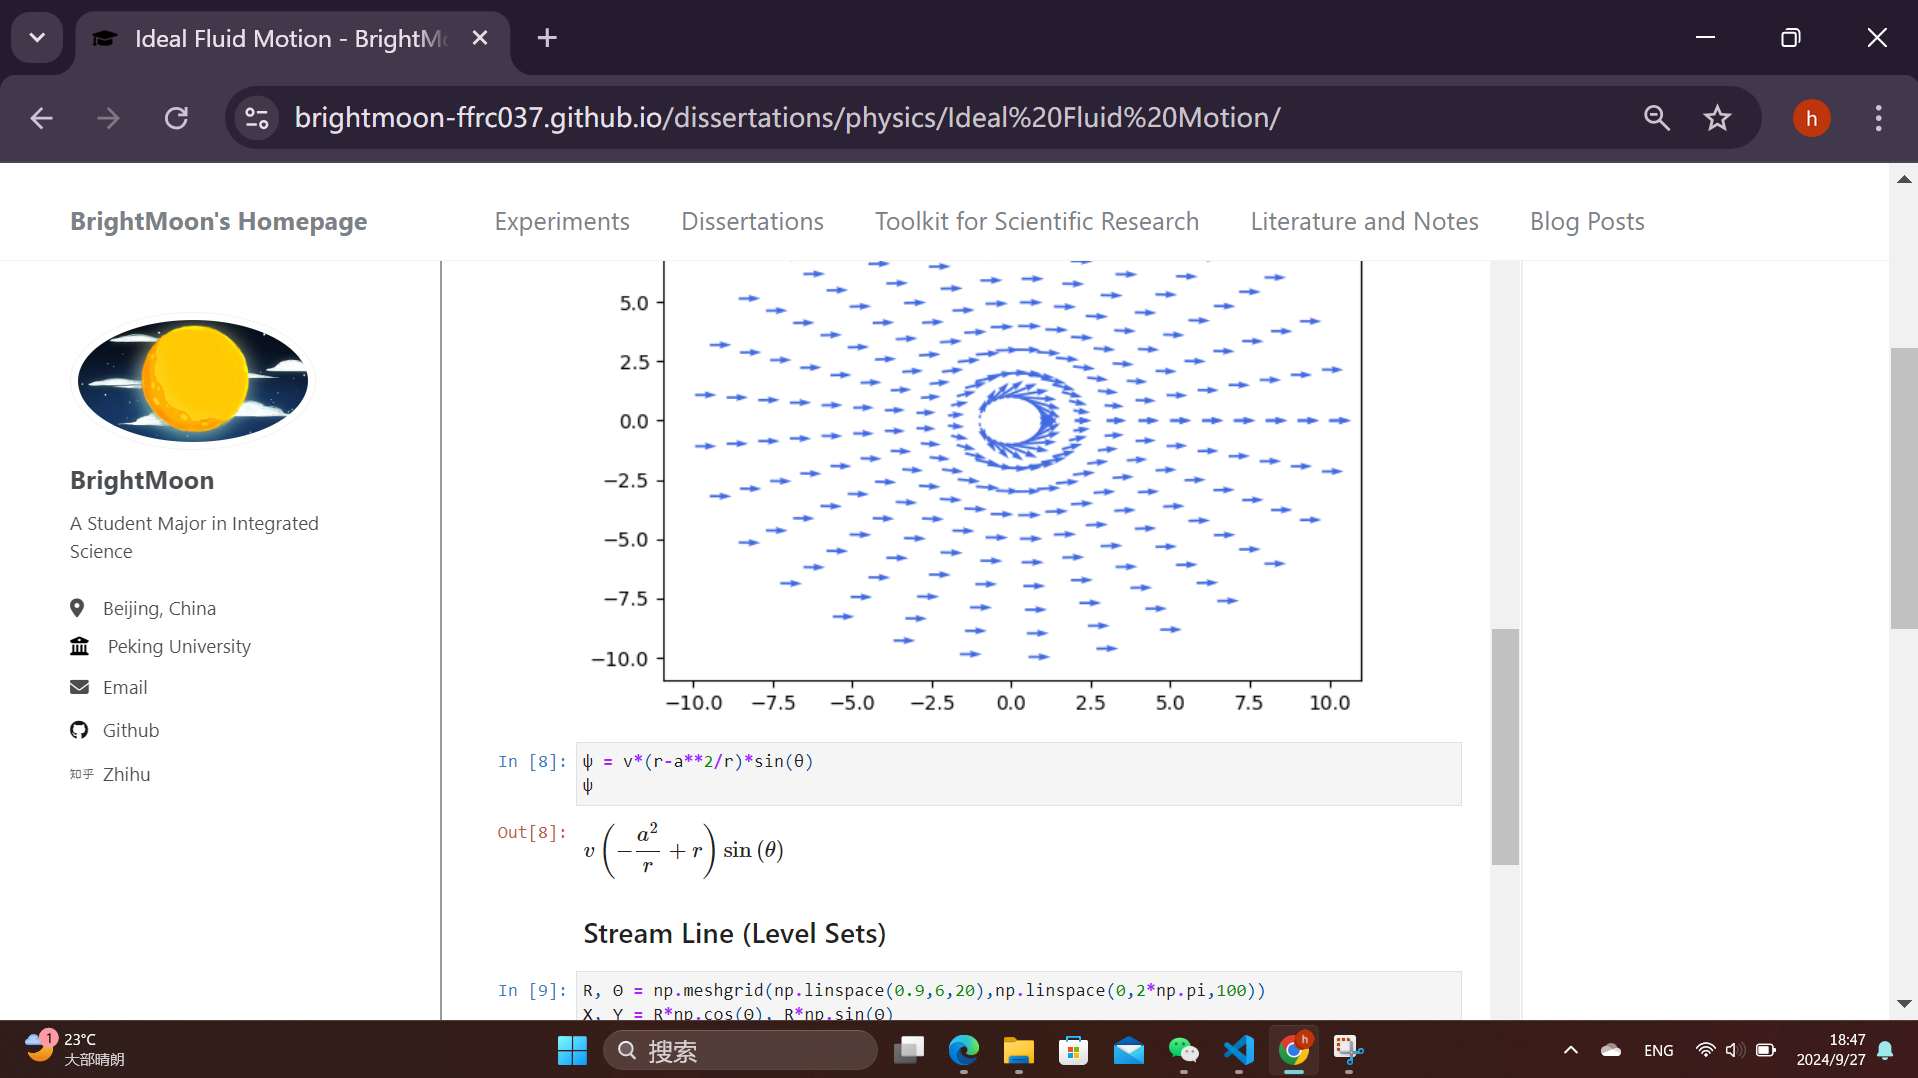
\includegraphics[width=0.7\linewidth]{../Figures/example 3.png}
    \caption{example 2}
    \label{example 2}
\end{figure}

% Table
\begin{table}
    \centering
    \begin{tabular}{|c|c|}\hline
        Column One & Column Two \\ \hline
        Content One & Content One\\ \hline
    \end{tabular}
    \caption{example 3}
    \label{example 3}
\end{table}

% List
\begin{itemize}
    \item item 1
    \item item 2
\end{itemize}


\bibliographystyle{plain}
\bibliography{references}
\end{document}